% !TeX encoding = UTF-8
% !TeX program = xelatex
\documentclass[12pt, a4paper]{article}
\usepackage[CheckSingle, CJKmath]{xeCJK}
\usepackage{amsthm}                             %定義,例題
\usepackage{amssymb}
\usepackage{array} % 製作表格必須的宏包
\usepackage{adjustbox}
\usepackage{amsmath, courier, listings, fancyhdr, graphicx}
\usepackage[english]{babel}
\usepackage{caption}
\usepackage{color}
\usepackage{CJKulem}
\usepackage{enumerate}
\usepackage{fontspec}
\usepackage{fancyhdr}                           %設定頁首頁尾
\usepackage{graphicx} % 插入圖片
\usepackage{geometry} 
\usepackage[utf8]{inputenc}
\usepackage{setspace}
\usepackage{tabularx} % 自動調整列寬的表格宏包
\usepackage{times}
\usepackage{titlesec}
\usepackage[x11names]{xcolor}

\setCJKfamilyfont{heiti}{Heiti TC}
\CJKfamily{heiti}
\setmainfont{Arial}
\setstretch{1.5}

\setmainfont[
    AutoFakeSlant,
    BoldItalicFeatures={FakeSlant},
    UprightFont={*},
    BoldFont={*-Bold}
]{Inconsolata}

\setmonofont[
    AutoFakeSlant,
    BoldItalicFeatures={FakeSlant},
    BoldFont={*-Bold}
]{Inconsolata}


\makeatletter
\lst@CCPutMacro\lst@ProcessOther {"2D}{\lst@ttfamily{-{}}{-{}}}
\@empty\z@\@empty
\makeatother
\lstset{                                        % Code顯示
    language=C++,                               % the language of the code
    basicstyle=\footnotesize\ttfamily,          % the size of the fonts that are used for the code
    numbers=left,                               % where to put the line-numbers
    numberstyle=\scriptsize,                    % the size of the fonts that are used for the line-numbers
    stepnumber=1,                               % the step between two line-numbers. If it's 1, each line  will be numbered
    numbersep=5pt,                              % how far the line-numbers are from the code
    backgroundcolor=\color{white},              % choose the background color. You must add \usepackage{color}
    showspaces=false,                           % show spaces adding particular underscores
    showstringspaces=false,                     % underline spaces within strings
    showtabs=false,                             % show tabs within strings adding particular underscores
    frame=false,                                % adds a frame around the code
    tabsize=2,                                  % sets default tabsize to 2 spaces
    captionpos=b,                               % sets the caption-position to bottom
    breaklines=true,                            % sets automatic line breaking
    breakatwhitespace=true,                     % sets if automatic breaks should only happen at whitespace
    escapeinside={\%*}{*)},                     % if you want to add a comment within your code
    morekeywords={*},                           % if you want to add more keywords to the set
    keywordstyle=\bfseries\color{Blue1},
    commentstyle=\itshape\color{Red1},
    stringstyle=\itshape\color{Green4},
}



\begin{document}
  \begin{center}
    {\Huge 資料結構實習} \\[2.5cm]
    {\Huge 11/17 作業報告} \\[1.5cm]
    {\Huge Stack 實作中序轉後序計算結果} \\ [4.5cm]
    \hspace{.6in}
    \begin{minipage}[t]{.4\linewidth}
      {\Large 班級:資訊二甲}\\[0.5cm]
      {\Large 學號:D1109023}\\[0.5cm]
      {\Large 姓名:楊孟憲}
    \end{minipage}    
  \end{center}

  \newpage

  \begin{samepage}
    \fontsize{16pt}{18pt} \selectfont  
    % 生成目錄
    \tableofcontents
    \normalfont
  \end{samepage}
  
  \newpage


  \section{\fontsize{20pt}{22pt}\selectfont 引言}
  \begin{samepage}
    \fontsize{16pt}{18pt} \selectfont
      \textbf{如何將中序轉為後續?} \\ 
      我們可以使用 Stack 的特質來實作,實作過程如下: 將 $(a + b) \times (a + d)$ 轉為後序。
      \begin{figure}[ht]
        \centering
        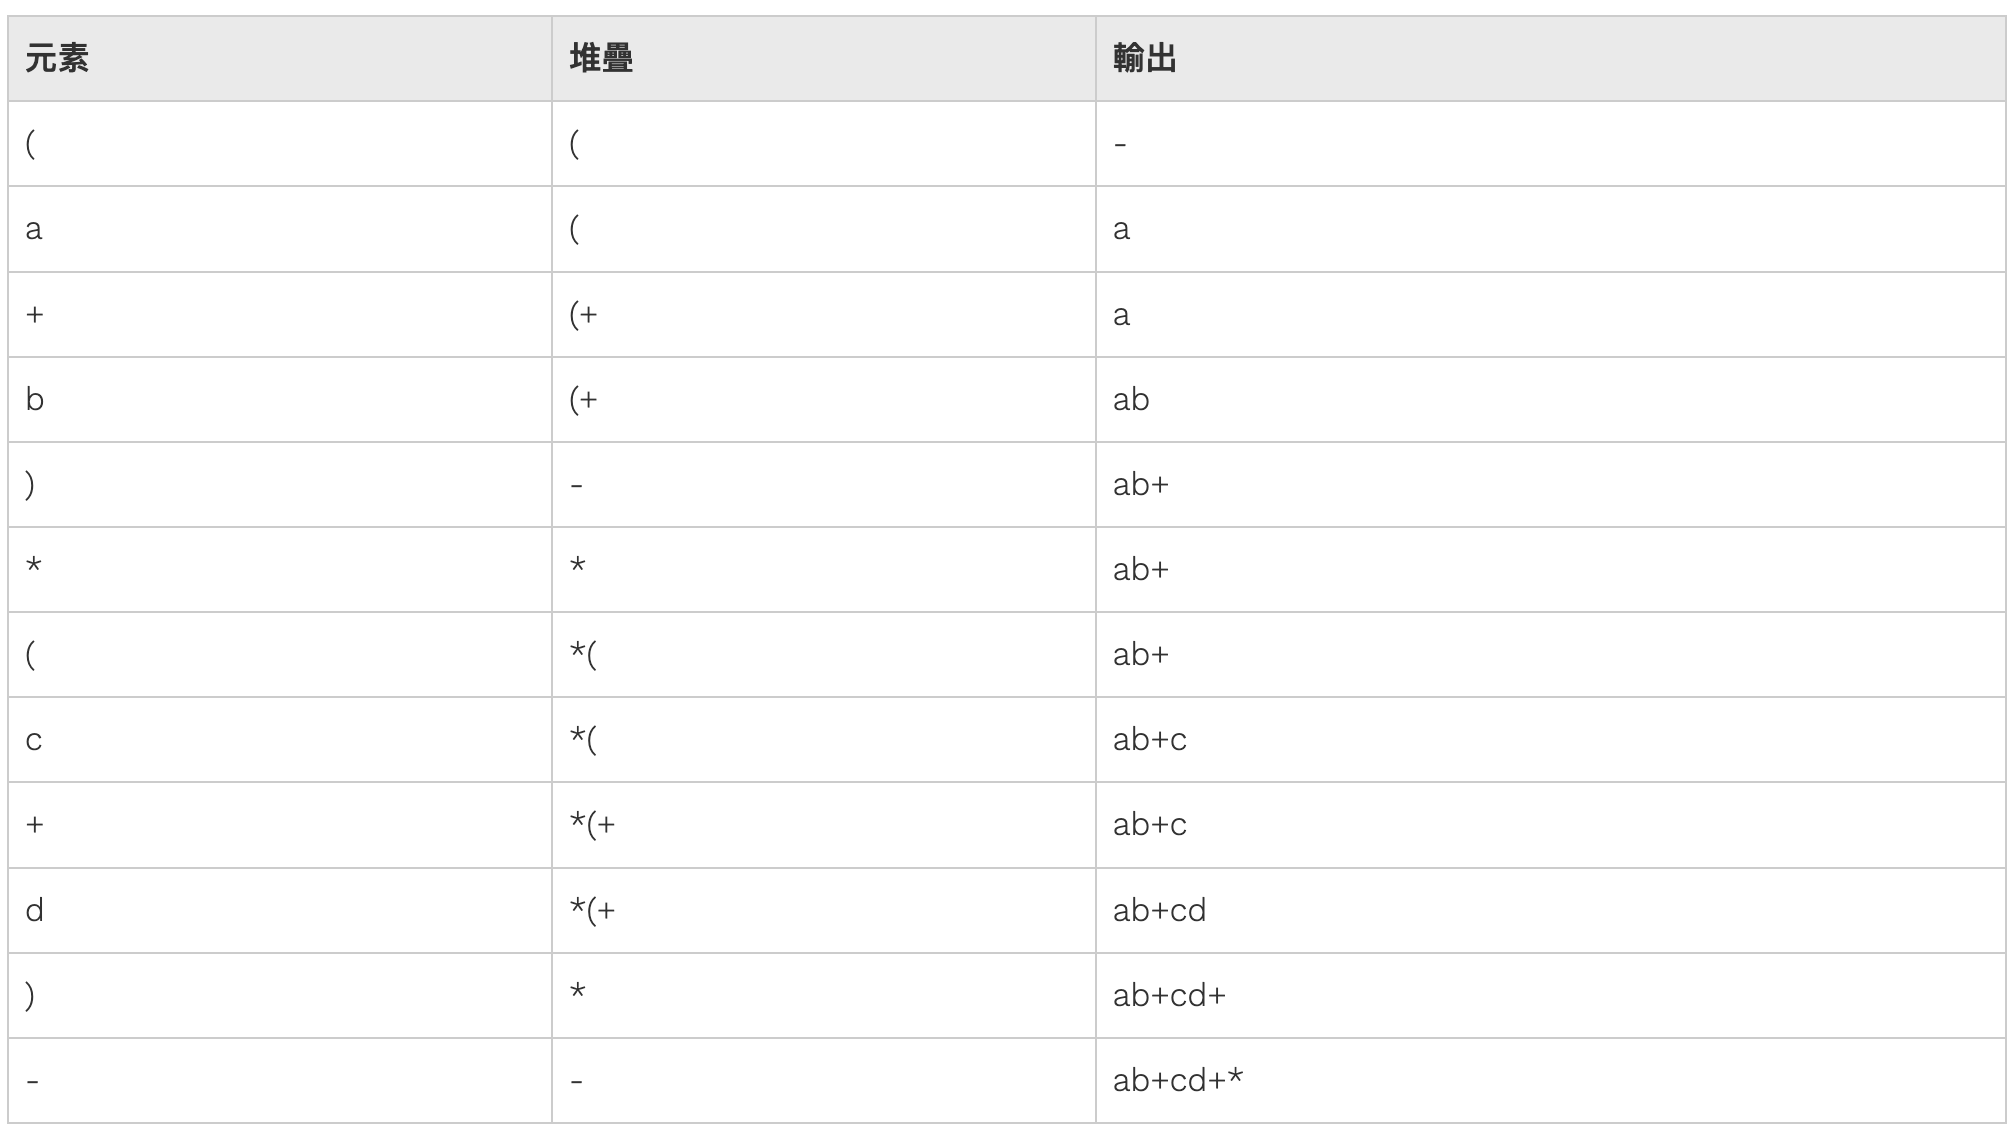
\includegraphics[width=0.8\textwidth]{./Image/screenshot01.png}
        \caption{圖一}
      \end{figure}
      \\
      \textbf{如何計算後序結果?} \\
      假設有一個後序為123*+,當遇到運算子時,就會將前兩個數字做運算,並解放回堆疊裡,以此類推。
      \begin{enumerate}
        \item 123*
        \item 16+
        \item 7
      \end{enumerate}
  \end{samepage}
  % 第一個章節

  \section{\fontsize{20pt}{22pt}\selectfont 題目敘述}
  \begin{samepage}
    \fontsize{16pt}{18pt} \selectfont
        \textbf{題意說明:} 讀入資料檔(1117hw.txt),檔案中是多個中序的運算式所組成的字串,
        請利用堆疊 (Stacks) 的原理來撰寫一個程式,將檔案中的字串分別讀入轉換成後序
        運算式,並且輸出運算結果。
  \end{samepage}
  % 第二個章節


  \section{\fontsize{20pt}{22pt}\selectfont 作法}
  % 第二章節的子章節
  \begin{samepage}
    \fontsize{16pt}{18pt} \selectfont
      宣告說明: st存放operator, res存放numbers, resProfix為後序結果, cnt為左括號數量。
      先將中序的運算子讀入,並且使用for迴圈遍歷每一個字元。當遇到數字的時候繼續累加數字。\\
      否則,當 haveNum == true 時,將now Push 進 res,如果沒有左括號(包含當前),判斷operator的優先層級(乘除大於加減),如果 Stack 裡的比當前的大就先拿出來做後序,
      如果當前字元是')'的話將st的運算符號拿出,直到左括號或堆疊為空為止(範例1)。\\
      迴圈執行完成後要將st剩餘的operator處理完(範例2) \\
      \textbf{範例1}  
      \lstinputlisting[language=C++]{./Contents/loop.cpp}
      \textbf{範例2}
      \lstinputlisting[language=C++]{./Contents/loop2.cpp}
      將中序轉換後會得到一個堆疊res以及一個字串resProfix,將res依照後序運算原理操作便可得到結果(範例3) \\
      \textbf{範例3}
      \lstinputlisting[language=C++]{./Contents/calculator.cpp}
      \normalfont
  \end{samepage}

  \section{\fontsize{20pt}{22pt}\selectfont 執行結果}
  % 第三個章節
      \fontsize{16pt}{18pt} \selectfont
        輸入輸出結果:(圖二)
        \begin{figure}[ht]
          \centering
          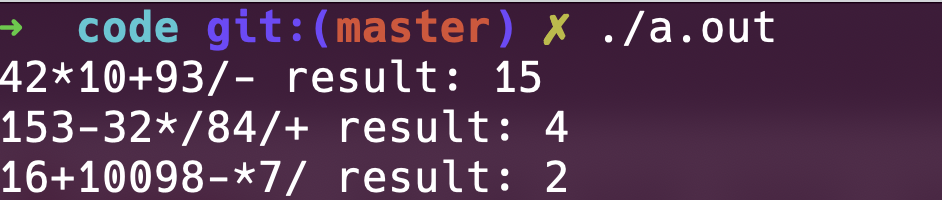
\includegraphics[width=0.8\textwidth]{./Image/screenshot.png}
          \caption{圖二}
        \end{figure}
      \normalsize

  \section{\fontsize{20pt}{22pt}\selectfont 心得與討論}
  \begin{samepage}
    \fontsize{16pt}{18pt} \selectfont
    這次的作業的先備知識需要先了解中序轉後序的原理以及利用後序計算結果,這讓我瞭解了如何例用Stack實作四則運算的題目,我覺得十分有挑戰性。
    實作過後我將結果丟到 ZeroJudge 上測試也沒有什麼問題,我覺得資料結構的能力以及對程式的手感有大幅提升。
    \normalfont
  \end{samepage}
  % 最後一個章節
\end{document}
